\textbf{Describe las principales características del enfoque de bases de datos y contrástalo con el
enfoque basado en hojas de cálculo. ¿En qué casos no tendría sentido utilizar una hoja de
cálculo? ¿En qué condiciones resultaría mejor opción utilizar las hojas de cálculo?}\\

Primero vamos a repasar un poco las diferencias entre estas 2 tecnologías para posteriormente ver en que situaciones nos conviene usar cada una.
\begin{center}
    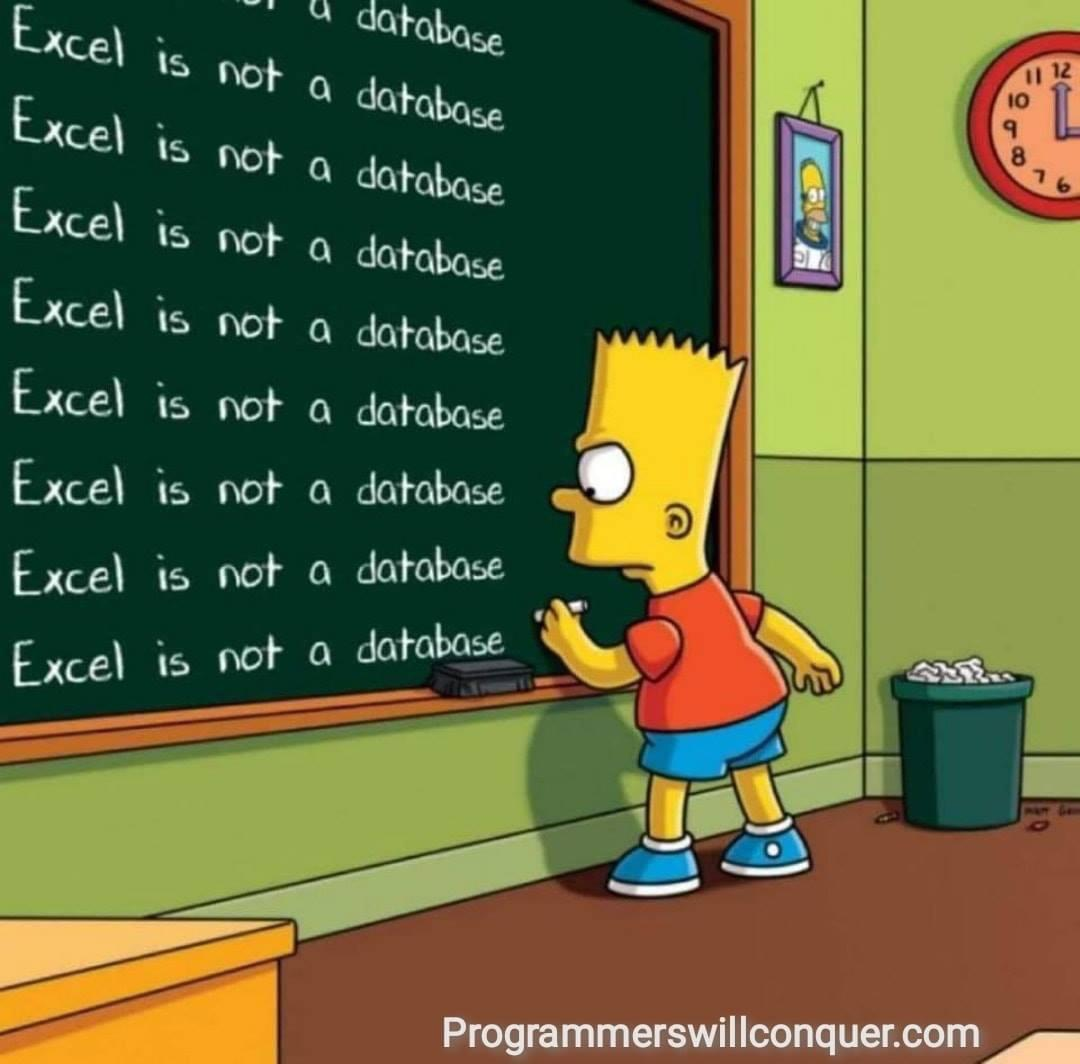
\includegraphics[width=6cm, height=6cm]{resources/chistocitojpg.jpg}\\
    \cite{RedditPost2020}\\
\end{center}

Hay que aclarar antes que nada que en realidad estos 2 sistemas manejadores de la información comparten mas cosas de las que las diferencian; esto pues ambas tienen un propósito similar, el de guardar datos de manera estructura y de manera superficial ambas guardan "tablas". Sin embargo es cuando nos metemos a ver los detalles de como funcionan y que nos dejan hacer que empezamos a ver el porque de usar cada.\\

\\

\begin{table}[h!]
    \centering
    \begin{tabular}{|p{4cm}||p{5.6cm}||p{5.6cm}|}
        \hline
        \textbf{Característica} &\textcolor{Green}{\textbf{Hojas de calculo}} & \textcolor{bibi}{\textbf{Bases de datos}} \\ \hline 
         Integridad de los datos & Es difícil de mantener & Es mas fácil mantener \\ \hline 
         Redundancia de datos & Es fácil guardar varias veces lo mismo por falta de atomicidad & Cuando esta bien hecha tiene pocos datos redundantes  \\ \hline
         Validez & Es difícil asegurar que nuestros datos tengan formato valido & Es algo mas fácil pasar nuestros datos a una forma normal  \\ \hline
         Visualización & Es fácil perder datos al tener que recorrer la pantalla & Con consultas SQL la maquina recorre por nosotros  \\ \hline 
         Rendimiento y capacidad & Como vimos en clase excel no puede tener mas de 1,048,576 filas por 16,384 columnas y la velocidad a la que procesa incluso estos datos es lenta & Oracle tiene un limite teórico de 8 exabytes aunque depende del hardware y la implementación, la velocidad esta ultra optimizada.  \\ \hline
         Seguridad & Suelen ser dificiles de proteger & Tienen estándares de seguridad y información distribuida  \\ \hline
    \end{tabular}
    \caption{Diferencias entre Hojas de Calculo y BDD \cite{BDDvsXML}}
    \label{tabla:ejemplo}
\end{table}

Entre otras cosas, como multiuso o su compatibilidad con la programación, las BDD parece como si le sacaran una gran ventaja a las hojas de calculo, entonces ¿porque usar hojas de calculo?\\

Bueno la verdad es que es una respuesta algo simple, y es que las bases de datos son muy caras y/o complejas para cosas simples, y es que para personas que no sean muy ávidas a la tecnología, utilizar una BDD y un SMBD es algo bastante complicado; además de esto, hay que aclarar que la mayoría bases de información no son realmente tan grandes, digamos que como persona es raro exceder las capacidades del poderosisimo excel y no es hasta que escalamos el problema a cientos de miles de registros o seamos una empresa que necesita ciertas de estas características que vale la pena empezar a usar una BDD.\\

Entonces de manera concisa cuando usar cada uno:\\\\
\textcolor{Green}{\textbf{Hojas de calculo}}\\
Mayormente para usos pequeños, de bajo coste y que no necesiten escalar, como puede ser tus finanzas personales, las de empresas o si se quiere una solución mas simple. Por ejemplo no tendría sentido intentar por ejemplo entrenar una IA con datos de hojas de calculo entre varias razones por el volumen de información, el rendimiento y la validez de la información.
\begin{center}
    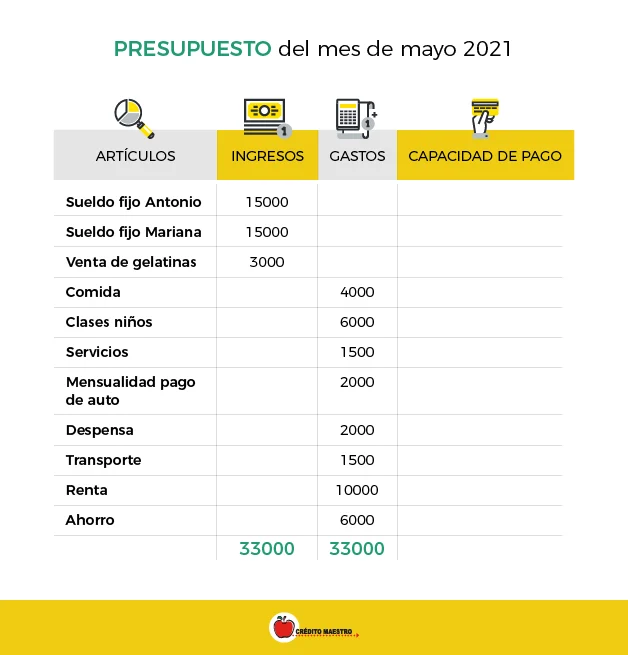
\includegraphics[width=6cm, height=6cm]{resources/HolaEXCELBB.png}\\
    \cite{FinanzasP}\\
\end{center}

\textcolor{bibi}{\textbf{Bases de datos}}\\
Son mejores para todo lo demás; no es cierto, básicamente cualquier aplicación de la vida real, todas las empresas medianas en adelante, cosas de gobierno, todo lo relacionado a data, mucho de lo que usa la IA, videojuegos entre muchos otros.\\\\
